\documentclass[12pt, a4paper, onepage, english,singlespacing, parskip]{scrartcl}

%\documentclass[
%11pt, 				% The default document font size, options: 10pt, 11pt, 12pt
%oneside, 			% Two side (alternating margins) for binding by default, uncomment to switch to one side
%chapterinoneline,	% Have the chapter title next to the number in one single line
%english, 			% ngerman for German
%singlespacing, 	% Single line spacing, alternatives: onehalfspacing or doublespacing
%draft, 			% Uncomment to enable draft mode (no pictures, no links, overfull hboxes indicated)
%nolistspacing, 	% If the document is onehalfspacing or doublespacing, uncomment this to set spacing in lists to single
%liststotoc, 		% Uncomment to add the list of figures/tables/etc to the table of contents
%toctotoc, 			% Uncomment to add the main table of contents to the table of contents
%parskip, 			% Uncomment to add space between paragraphs
%nohyperref, 		% Uncomment to not load the hyperref package
%headsepline, 		% Uncomment to get a line under the header
%]{scrartcl or scrreprt or scrbook} % The class file specifying the document structure

\usepackage{lmodern} 		% Diese beiden packages sorgen für echte 
\usepackage[T1]{fontenc}	% Umlaute.

\usepackage{amssymb, amsmath, color, dsfont, graphicx, float, setspace, tipa}
\usepackage[utf8]{inputenc} 
\usepackage[english]{babel}
\usepackage[pdfpagelabels,
			pdfstartview = FitH,
			bookmarksopen = true,
			bookmarksnumbered = true,
			linkcolor = black,
			plainpages = false,
			hypertexnames = false,
			citecolor = black,
			breaklinks]{hyperref}
\usepackage{url}
\usepackage{longtable} 		% Tables along multiple pages
\usepackage{caption}
\captionsetup{font=small,labelfont=bf, format=plain, justification=centering}
\allowdisplaybreaks 		% allows page breaks in align/equation environment

\usepackage{authblk} 		% titlepage stuff
\usepackage[titletoc, title]{appendix}

\usepackage{newclude} 		% use \include*{file} instead \include{} to omit pagebreak after include




%===================
% BIBLIOGRAPHY
%===================

\usepackage[]{natbib}
\bibliographystyle{unsrtnat}


%DONT FORGET TO COMPILE THE BIBLIOGRAPHY WITH BIBTEX WHEN CHANGES ARE MADE.



%--------------------------------------------
%     OPTIONAL
%--------------------------------------------



%% Change font
%\newcommand{\changefont}[3]{
%\fontfamily{#1} \fontseries{#2} \fontshape{#3} \selectfont}
%\changefont{ppl}{m}{n} nach \begin{document} einsetzen

% Fig. instead of Figure, Tab. instead of Table
%\usepackage[footnotesize]{caption2}
%\addto\captionsenglish{\renewcommand{\figurename}{Fig.}}
%\addto\captionsngerman{\renewcommand{\figurename}{Fig.}}
%\renewcommand{\tablename}{Tab.}%

%\pagestyle{headings} % Write headings on each page

%\usepackage{chngcntr} \counterwithout{figure}{section} % Integer only figure numbers, ignoring chapter numbers






%-----------------------------------------------
% FORMAT TITLE
%-----------------------------------------------


% Set fonts of document parts
\setkomafont{title}{\rmfamily\bfseries\boldmath}
\addtokomafont{section}{\rmfamily\bfseries\boldmath}
\addtokomafont{subsection}{\rmfamily\bfseries\boldmath}
\addtokomafont{subsubsection}{\rmfamily\bfseries\boldmath}
\addtokomafont{disposition}{\rmfamily} % table of contents and stuff
\setkomafont{descriptionlabel}{\rmfamily\bfseries\boldmath}



% add my definitions here
%==============================================
% This file contains my definitions and
% newcommands. Makes things easy to copypaste
% between projects.
%==============================================


%--------------------------------------------
% Math Stuff
%--------------------------------------------

\newcommand{\corresponds}{\mathrel{\widehat{=}}}       % equals with hat

\newcommand {\arctanh}{\mathrm{arctanh}}               % Atanh
\newcommand{\arccot}{\mathrm{arccot }}                 % Acotanh

\newcommand{\limz}[1]{\lim\limits_{#1 \rightarrow 0}}  % Limes of something towards zero

\newcommand{\bm}{\boldmath}                            % Bold font in math
\newcommand{\dps}{\displaystyle}                                               

\newcommand{\e}{\mbox{e}}                              % e noncursive in math mode

\newcommand{\del}{\partial}                            % partial diff operator
\newcommand{\de}{\mathrm{d}}                           % differential d
\newcommand{\D}{\mathrm{d}}                            % differential d
\newcommand{\GRAD}{\mathrm{grad}\ }                    % gradient
\newcommand{\DIV}{\mathrm{div}\ }                      % divergence
\newcommand{\ROT}{\mathrm{rot}\ }                      % rotation

\newcommand{\CONST}{\mathrm{const.\ }}                 % constant
\newcommand{\var}{\mathrm{var}}                        % variance

\newcommand{\g}{^\circ}                                % degrees
\newcommand{\degr}{^\circ}                             % degrees

\newcommand{\msol}{M_\odot}                            % solar mass


\newcommand{\x}{\mathbf{x}}                            % x vector
\newcommand{\xdot}{\dot{\mathbf{x}}}                   % x dot vector
\newcommand{\xddot}{\ddot{\mathbf{x}}}                 % x doubledot vector
\newcommand{\R}{\mathbf{r}}                            % r vector
\newcommand{\rdot}{\dot{\mathbf{r}}}                   % r dot vector
\newcommand{\rddot}{\ddot{\mathbf{r}}}                 % r doubledot vector
\newcommand{\vel}{\mathbf{v}}                          % v vector
\newcommand{\V}{\mathbf{v}}                            % v vector
\newcommand{\vdot}{\dot{\mathbf{v}}}                   % v dot vector
\newcommand{\vddot}{\ddot{\mathbf{v}}}                 % v doubledot vector

\newcommand{\dete}{\mathrm{d}t}                        % dt
\newcommand{\delte}{\del t}                            % partial t
\newcommand{\dex}{\mathrm{d}x}                         % dx
\newcommand{\delx}{\del x}                             % partial x
\newcommand{\der}{\mathrm{d}r}                         % dr
\newcommand{\delr}{\del r}                             % partial r






%-----------------------------------------------
% Work related / project specific math stuff
%-----------------------------------------------

\newcommand{\Aij}{$\mathbf{A}_{ij}$}	% A_ij
\newcommand{\Aijm}{\mathbf{A}_{ij}}		% A_ij math
\newcommand{\U}{\mathbf{U}}				% State vector
\newcommand{\F}{\mathbf{F}}				% Flux tensor
\newcommand{\psitilde}{\tilde{\psi}}	% psi tilde










%----------------------------------
% Redefinitions
%----------------------------------


% replace \sum with \sum\limits
\let\oldsum\sum
\renewcommand{\sum}{\oldsum\limits}






%-----------------------------------
% Shortcuts
%-----------------------------------

% shortcut for TODO box
%		usage: \todo{Your text here}
\newcommand{\todo}[1]{\begin{mdframed}[style=todo,frametitle={TODO}] #1 \end{mdframed}}


% quickly insert a figure without a caption
% 		usage: \quickfig{filename}{label}
\newcommand{\quickfig}[2]{
       \begin{figure}[H]
               \includegraphics[width=\textwidth]{#1}
               \caption{\label{#2}}
       \end{figure}
}












%-----------------------------------------------
% TEXT IN BOXES
%-----------------------------------------------
 
\usepackage[framemethod=TikZ]{mdframed}

% New Colors (needs to be after usepackage mdframed)
\definecolor{babyblueeyes}{rgb}{0.63, 0.79, 0.95}
\definecolor{ashgrey}{rgb}{0.7, 0.75, 0.71}
\definecolor{caribbeangreen}{rgb}{0.0, 0.8, 0.6}
\definecolor{bittersweet}{rgb}{1.0, 0.44, 0.37}

\mdfdefinestyle{todo}{%
       %rightline=true,
       innerleftmargin=10,
       innerrightmargin=10,
       %frametitlerule=true,
       %frametitlerulecolor=black,
       frametitlebackgroundcolor=babyblueeyes,
       frametitlerulewidth=2
}


\mdfdefinestyle{eyecatcher}{%
       %rightline=true,
       innerleftmargin=10,
       innerrightmargin=10,
       %frametitlerule=true,
       %frametitlerulecolor=black,
       frametitlebackgroundcolor=bittersweet,
       frametitlerulewidth=2
}









%---------------------------------------------------
% Journal abbreviations
%---------------------------------------------------

%  http://adsabs.harvard.edu/abs_doc/aas_macros.sty
%
%  These Macros are taken from the AAS TeX macro package version 5.2
%  and are compatible with the macros in the A&A document class
%  version 7.0
%  Include this file in your LaTeX source only if you are not using
%  the AAS TeX macro package or the A&A document class and need to
%  resolve the macro definitions in the TeX/BibTeX entries returned by
%  the ADS abstract service.
%
%  If you plan not to use this file to resolve the journal macros
%  rather than the whole AAS TeX macro package, you should save the
%  file as ``aas_macros.sty'' and then include it in your LaTeX paper
%  by using a construct such as:
%	\documentstyle[11pt,aas_macros]{article}
%
%  For more information on the AASTeX and A&A packages, please see:
%       http://journals.aas.org/authors/aastex.html	
%       ftp://ftp.edpsciences.org/pub/aa/readme.html
%  For more information about ADS abstract server, please see:
%       http://adsabs.harvard.edu/ads_abstracts.html
%

% Abbreviations for journals.  The object here is to provide authors
% with convenient shorthands for the most "popular" (often-cited)
% journals; the author can use these markup tags without being concerned
% about the exact form of the journal abbreviation, or its formatting.
% It is up to the keeper of the macros to make sure the macros expand
% to the proper text.  If macro package writers agree to all use the
% same TeX command name, authors only have to remember one thing, and
% the style file will take care of editorial preferences.  This also
% applies when a single journal decides to revamp its abbreviating
% scheme, as happened with the ApJ (Abt 1991).


\makeatletter

\let\jnl@style=\rm
\def\ref@jnl#1{{\jnl@style#1}}

\def\aj{\ref@jnl{AJ}}                   % Astronomical Journal
\def\actaa{\ref@jnl{Acta Astron.}}      % Acta Astronomica
\def\araa{\ref@jnl{ARA\&A}}             % Annual Review of Astron and Astrophys
\def\apj{\ref@jnl{ApJ}}                 % Astrophysical Journal
\def\apjl{\ref@jnl{ApJ}}                % Astrophysical Journal, Letters
\def\apjs{\ref@jnl{ApJS}}               % Astrophysical Journal, Supplement
\def\ao{\ref@jnl{Appl.~Opt.}}           % Applied Optics
\def\apss{\ref@jnl{Ap\&SS}}             % Astrophysics and Space Science
\def\aap{\ref@jnl{A\&A}}                % Astronomy and Astrophysics
\def\aapr{\ref@jnl{A\&A~Rev.}}          % Astronomy and Astrophysics Reviews
\def\aaps{\ref@jnl{A\&AS}}              % Astronomy and Astrophysics, Supplement
\def\azh{\ref@jnl{AZh}}                 % Astronomicheskii Zhurnal
\def\baas{\ref@jnl{BAAS}}               % Bulletin of the AAS
\def\bac{\ref@jnl{Bull. astr. Inst. Czechosl.}}
                % Bulletin of the Astronomical Institutes of Czechoslovakia 
\def\caa{\ref@jnl{Chinese Astron. Astrophys.}}
                % Chinese Astronomy and Astrophysics
\def\cjaa{\ref@jnl{Chinese J. Astron. Astrophys.}}
                % Chinese Journal of Astronomy and Astrophysics
\def\icarus{\ref@jnl{Icarus}}           % Icarus
\def\jcap{\ref@jnl{J. Cosmology Astropart. Phys.}}
                % Journal of Cosmology and Astroparticle Physics
\def\jrasc{\ref@jnl{JRASC}}             % Journal of the RAS of Canada
\def\memras{\ref@jnl{MmRAS}}            % Memoirs of the RAS
\def\mnras{\ref@jnl{MNRAS}}             % Monthly Notices of the RAS
\def\na{\ref@jnl{New A}}                % New Astronomy
\def\nar{\ref@jnl{New A Rev.}}          % New Astronomy Review
\def\pra{\ref@jnl{Phys.~Rev.~A}}        % Physical Review A: General Physics
\def\prb{\ref@jnl{Phys.~Rev.~B}}        % Physical Review B: Solid State
\def\prc{\ref@jnl{Phys.~Rev.~C}}        % Physical Review C
\def\prd{\ref@jnl{Phys.~Rev.~D}}        % Physical Review D
\def\pre{\ref@jnl{Phys.~Rev.~E}}        % Physical Review E
\def\prl{\ref@jnl{Phys.~Rev.~Lett.}}    % Physical Review Letters
\def\pasa{\ref@jnl{PASA}}               % Publications of the Astron. Soc. of Australia
\def\pasp{\ref@jnl{PASP}}               % Publications of the ASP
\def\pasj{\ref@jnl{PASJ}}               % Publications of the ASJ
\def\rmxaa{\ref@jnl{Rev. Mexicana Astron. Astrofis.}}%
                % Revista Mexicana de Astronomia y Astrofisica
\def\qjras{\ref@jnl{QJRAS}}             % Quarterly Journal of the RAS
\def\skytel{\ref@jnl{S\&T}}             % Sky and Telescope
\def\solphys{\ref@jnl{Sol.~Phys.}}      % Solar Physics
\def\sovast{\ref@jnl{Soviet~Ast.}}      % Soviet Astronomy
\def\ssr{\ref@jnl{Space~Sci.~Rev.}}     % Space Science Reviews
\def\zap{\ref@jnl{ZAp}}                 % Zeitschrift fuer Astrophysik
\def\nat{\ref@jnl{Nature}}              % Nature
\def\iaucirc{\ref@jnl{IAU~Circ.}}       % IAU Cirulars
\def\aplett{\ref@jnl{Astrophys.~Lett.}} % Astrophysics Letters
\def\apspr{\ref@jnl{Astrophys.~Space~Phys.~Res.}}
                % Astrophysics Space Physics Research
\def\bain{\ref@jnl{Bull.~Astron.~Inst.~Netherlands}} 
                % Bulletin Astronomical Institute of the Netherlands
\def\fcp{\ref@jnl{Fund.~Cosmic~Phys.}}  % Fundamental Cosmic Physics
\def\gca{\ref@jnl{Geochim.~Cosmochim.~Acta}}   % Geochimica Cosmochimica Acta
\def\grl{\ref@jnl{Geophys.~Res.~Lett.}} % Geophysics Research Letters
\def\jcp{\ref@jnl{J.~Chem.~Phys.}}      % Journal of Chemical Physics
\def\jgr{\ref@jnl{J.~Geophys.~Res.}}    % Journal of Geophysics Research
\def\jqsrt{\ref@jnl{J.~Quant.~Spec.~Radiat.~Transf.}}
                % Journal of Quantitiative Spectroscopy and Radiative Transfer
\def\memsai{\ref@jnl{Mem.~Soc.~Astron.~Italiana}}
                % Mem. Societa Astronomica Italiana
\def\nphysa{\ref@jnl{Nucl.~Phys.~A}}   % Nuclear Physics A
\def\physrep{\ref@jnl{Phys.~Rep.}}   % Physics Reports
\def\physscr{\ref@jnl{Phys.~Scr}}   % Physica Scripta
\def\planss{\ref@jnl{Planet.~Space~Sci.}}   % Planetary Space Science
\def\procspie{\ref@jnl{Proc.~SPIE}}   % Proceedings of the SPIE

\let\astap=\aap
\let\apjlett=\apjl
\let\apjsupp=\apjs
\let\applopt=\ao


\makeatother





%---------------------
%  Metadata
%---------------------

 \title[shortform]{Title}
%     Titel of the presentations
 \subtitle[shortform-subtitle]{Subtitile}
%     Subtitle
 \author[M. Ivkovic]{Mladen Ivkovic}
%     Set author
 \institute[EPFL]{LASTRO \\ \'Ecole Polytechnique F\'ed\'erale de Lausanne}
%     Institute
 \date[17.09.19]{17. September 2019}
%	  Date of presentation. Alternatively you can use \today to set compilation time date automatically.
% \logo{\pgfimage[width=2cm,height=2cm]{mylogo}}
%     Add mylogo.pdf (bzw. mylogo.png, mylogo.jpg, mylogo.mps if you're using pdftex as Backend) as the logo on all slides, here using the package pgf.
% \titlegraphic{\includegraphics[width=2cm,height=2cm]{mylogo}}
%	  Add mylogo.pdf/png/jpg file as the logo only on the title packe using the graphicx package









%===================================================================================
%===================================================================================
%
%
%
% \begin{frame}[Overlay-actrions][options]{Title}{Subtitle}
% 
%Overlay-actions
%	Overlay-actions set the default overlay actions of all environments within the 
%	frame, which allow action-specifications, e.g. \item in lists and blocks.
%	Overlays are 'animations' for elements on a slide, e.g. items appearing one after 
%	the other.
%
% 
%     <+->
%			makes the elements appear one by one.
% 
% options
% 
%     allowdisplaybreaks
%			allows a page break in multi-line equations. Works only together with option
%			allowframebreaks
%
%     allowframebreaks
%			automatically distribute the contents on multiple slides if it doesn't fit
%			on only one. However this disables overlays.
%
%     b,c,t
%			aligns frame to (b)ottom, (t)op or (c)enter
%
%     fragile
%			necessary for sourse text environments, e.g. verbatim
%
%     label=name
%			set a name for the frame so you can call it again later with \againframe{label}
%
%     plain
%			suppresses header, footer, and sidebar.
%
%     squeeze
%			minimizes vertical spacings as far as possible to make more content possible
%			on a slide
%
% 
%===================================================================================
%===================================================================================




\begin{document}


\begin{frame}{}
	\titlepage
\end{frame}


\begin{frame}{Outline}\label{tableofcontents}
   \tableofcontents
\end{frame}






%=======================================
\section{Section Name}
%=======================================

\begin{frame}
	\frametitle{Test Frametitle}
	\framesubtitle{Test yo}

    \begin{itemize}
		\item Test
		\item Test 2
		\item Test 3
    \end{itemize}

    \begin{description}
		\item[${G_3}'$:] Text goes here.
		\item WTF
		\item [Item Name] Description
    \end{description}
\end{frame}









%=======================================
\section{Blocks}
%=======================================


\begin{frame}
	\frametitle{blocks}

    \begin{block}{simple block title}
        Simple block text
    \end{block}
    
    \begin{exampleblock}{example block title}
         example block text
    \end{exampleblock}
   
    \begin{alertblock}{alert block title}
         alert block text
    \end{alertblock}
    
\end{frame}












%=========================================================
\section{Proof, Definitions, Lemmata, Remarks}
%=========================================================


\begin{frame}[fragile] % need fragile for verbatim
	\frametitle{Proofs etc}

    \begin{proof}
        Proof
    \end{proof}
    
    \begin{lemma}[XY -- A dual zu YX]
        Lemma
    \end{lemma}
    
    \begin{theorem}[T -- after Tarski]
        Theorem
    \end{theorem}
    
     \begin{rem}
		remark: first set
		  \begin{verbatim}
		    \newtheorem*{rem}{Remark}
		  \end{verbatim}
		  in preamble! 
     \end{rem}
\end{frame}








%=========================================================
\section{Overlays}
%=========================================================


\begin{frame}
	\frametitle{Overlays}
   \begin{itemize}
        \item Start
        \item<2-> so it follows
        \item<3-> then this
        \item<4-> then that
   \end{itemize}
\end{frame}











%=========================================================
\section{Two Columns}
%=========================================================

\begin{frame}
	\frametitle{Two column stuff}
    \begin{columns}
         \column{.55\textwidth}
                 \pgfimage[width=\textwidth]{figures/test.jpg}
         \column{.45\textwidth}
                 \begin{enumerate}
                 \item Start
                 \item Stop
                 \end{enumerate}
    \end{columns}
\end{frame}
















%=========================================================
\section{Images}
%=========================================================





%=======================================
\subsection{Two images}
%=======================================


\begin{frame}{Two images}
\begin{figure}[!htb]
	\centering
	\minipage{0.4\textwidth}
		\fbox{
\includegraphics[height=3cm, keepaspectratio]{figures/test.jpg}}%
		\caption{
			I really don't 
			\label{fig:noidea1}
		}%
	\endminipage\hspace{1cm}   
	%
	\minipage{0.4\textwidth}
		\fbox{
\includegraphics[height=3cm, keepaspectratio]{figures/test.jpg}}%
		\caption{
			\smash{indeed I don't} 
			\label{fig:noidea2}
		}%
	\endminipage
\end{figure}
\end{frame}










%====================================
\subsection{Full Page Image}
%====================================




{
	\setbeamertemplate{background}
	{
		\vbox to \paperheight{
			\vfil\hbox to \paperwidth{
				\hfil
\includegraphics[width=\paperwidth]{figures/test.jpg}
			\hfil}
		}
	}
	\begin{frame}[plain]
		\frametitle{Full Page Image}
	\end{frame}
}





\begin{frame}[fragile]
	\frametitle{Small caption for big image}
	\begin{figure}[!htb]
		\begin{center}
			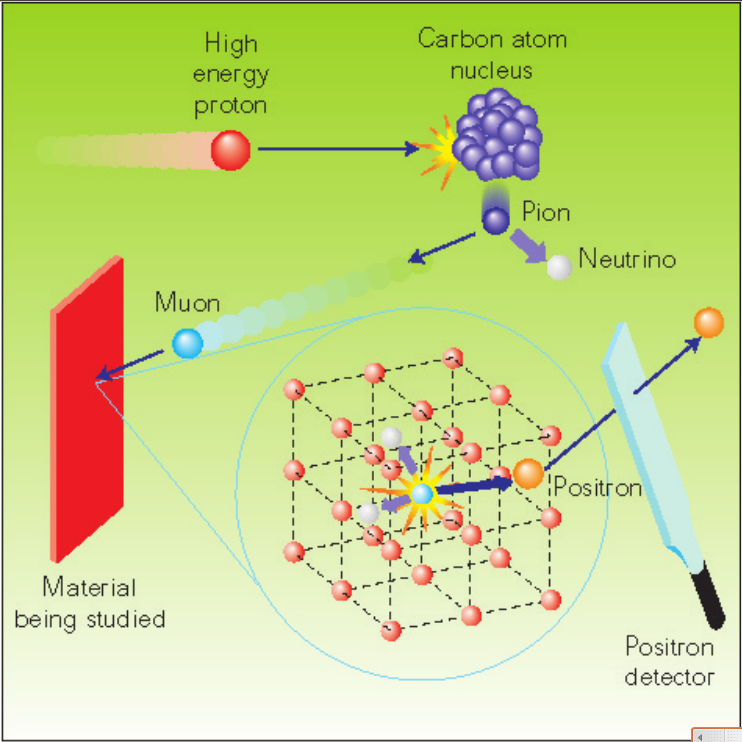
\includegraphics[height=6cm, keepaspectratio]{figures/musr_general_principle.png}%
			\caption*{  \setlength{\baselineskip}{6pt}
				{\tiny 
					Dalmas de Réotier, Pierre (2010): \textit{ 						
						Introduction to muon spin rotation and relaxation.
					}
					[Online]. Availible: \url{
						http://inac.cea.fr/Pisp/pierre.dalmas-de-reotier/introduction_muSR.pdf
					}
				}
			}%
		\end{center}
	\end{figure}          
\end{frame}






















%====================================
\subsection{Math}
%====================================




\begin{frame}
	\frametitle{Math}
	\begin{align}
			 f(z) &= 
			 	\lim\limits_{x\rightarrow \infty} \frac{\sin x}{x} = 0\\
		 	 \binom{a}{n} &= 
		 	 	\frac{a!}{(a-n)! n!}\\
		 	 \nonumber \int(z) dz &=  
		 	 	\frac14 \left[ \int\frac{e^{ia(u + 1)}}{u} du - \int\frac{e^{ia(u + 1)}}{u + 2}du   \right]\\[1em]
		 	 & \overset{z = 1 \Rightarrow u = 0}=  
		 	 	\frac{e^{i a}}{4} \left[\vphantom{ \int\limits_{\pi}^0} \smash{ \underbrace{\frac{\overbrace{e^{ia \epsilon e^{i \varphi}}}^{\rightarrow 1}} {\epsilon e^{i \varphi}} i \epsilon e^{i \varphi}}_{\rightarrow i}  d \varphi            - \int\limits_{\pi}^0 \underbrace{\frac{\overbrace{e^{ia \epsilon e^{i \varphi}}}^{\rightarrow 1}} {\underbrace{\epsilon e^{i \varphi}}_{\rightarrow 0} + 2} \underbrace{i \epsilon e^{i \varphi}}_{\rightarrow 0}}_{\rightarrow 0}  d \varphi  }\right]\\[2em]
		 	 %	
		 	 %
		 	 2 + 2 &= 4 \ \text{some more space after this line please.}\\[4em]\nonumber
	\end{align}
\end{frame}













%=========================================================
\section{Citations and References}
%=========================================================


\begin{frame}{Citations and References}
    \cite{AHF}
    
    \parencite{AMR}
    
    \renewcommand*{\bibfont}{\footnotesize}
    \printbibliography[]    
\end{frame}






\end{document}
